%!TEX root = ../thesis.tex

\chapter{Fundamentals}
\label{cha:fundamentals}
In this chapter, I present the fundamental natural language processing concepts relevant to this thesis (\textit{word embedding}) and previous work focused on integrating their capabilities into relational database management systems (\textit{FREDDY - Fast Word Embeddings in Database Systems}).

\section{Word Embedding}
\textit{Word embedding} is considered one of the key breakthroughs in using deep learning methods to challenge natural language processing problems \cite{we-mlm}. Here, I provide a short overview of its concept and list several of its practical applications.

\subsection{Definitions and Concept}
\begin{figure}[b]
	\centering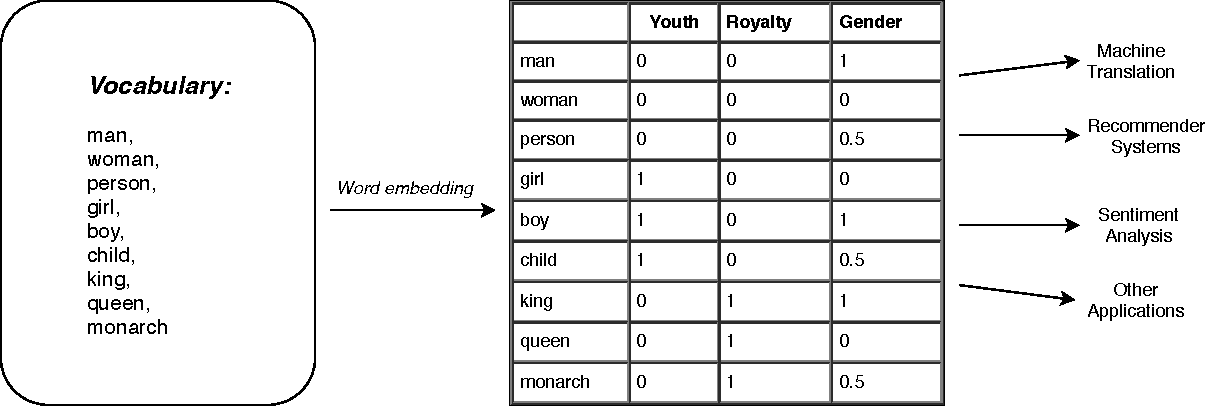
\includegraphics[width=\textwidth,keepaspectratio]{word_embedding.pdf}
	\caption{A figure illustrating word embedding and its applications.}
	\label{fig:word_embedding}
\end{figure}
The term \textit{word embedding} denotes a number of language modeling and feature learning techniques used in natural language processing. Their common feature is that they map words or phrases from a vocabulary to vectors of real numbers in a vector space. Generating the word-vector mappings may be done in different ways, e.g., by using neural networks, probabilistic models or explicit representation in terms of the context in which words appear. Most commonly, large text corpora are processed by neural networks to generate the word vectors, which is a time-consuming task. Because of this, word embeddings data sets readily available on the Internet (listed in Section \ref{sec:datasets}) were used for this project's purposes. 

The term \textit{word embeddings} is also used for the vectors generated using such methods. Each word embedding corresponds to a single word or phrase of the input corpus. They capture the semantical, morphological, contextual or hierarchical information contained in the corpus' vocabulary. Depending on the technique used, they may reflect the structure of a word in terms of morphology, serve as a word-context representation or show the relationship between a set of documents and the terms contained in them \cite{we-intro}. Each element of a vector represents a different aspect, or feature, of a word. Word embedding vectors are usually dense and low-dimensional (up to several hundred dimensions). The idea behind using dense vectors is generalization, which is hard to obtain when using a sparse representation. For example, in \textit{one-hot encoding}, a word-representing vector has a length equal to the vocabulary's size and consists only of zeros, except for a one in the position standing for the word. This representation cannot encode the complex semantical relations between words, as the number of features of a word is much smaller than the size of the vocabulary. Thus, a dense representation such as word embedding is well-suited to capture the likeness between words having similar features \cite{goldberg2017neural} \cite{bengio2003neural}. This results in words used in a similar way also having a similar word embedding representation (see Figure \ref{fig:word_embedding}, where words are represented as three-dimensional vectors based on deduced features).

\subsection{Applications}
Word embeddings have found many applications in various fields. As word embeddings are numerical representations of similarities between words, vector operations (henceforth called \textit{word embedding operations}) can be used to manipulate them and grant insights into previously unavailable semantic information. As a basic example, adding the vector for \textit{king} to the vector for \textit{woman}, then subtracting the vector for \textit{man} from the sum may result in a vector corresponding to \textit{queen}.

The real-valued vector space into which words were embedded comes with the notions of distance and angle. These notions also extend to embedded words and provide information, e.g., about relationships between them and their similarity \cite{we-intro-huang}. For example, a team at Google Inc. developed an algorithm called \textit{word2vec} which learned to distinguish between gendered forms of nouns and found out the difference between singular and plural forms of nouns in English. The same algorithm also discovered the existence of a relationship between a country and its capital. Interestingly, the team developing \textit{word2vec} also found that the learned structure for one language often correlates to that of another language. This opens new possibilities of using word embeddings for \textit{machine translation}, a traditionally challenging problem \cite{mikolov2013exploiting}. 

Word embeddings can be used in recommendation algorithms by various businesses. Among others, the music streaming application \textit{Spotify} uses them to provide new music recommendations to its users \cite{spotify-word2vec}. Furthermore, Google's search engine makes use of \textit{word2vec} as part of its recently developed RankBrain search algorithm \cite{rankbrain-seo}.

\textit{Sentiment analysis}, the process of determining the emotional tone behind textual information, is another field of application of word embeddings. One and the same word may carry a different connotation depending on the context of its use. For example, \textit{soft} may be used in a negative way when talking about a sport player's performance, but have a positive meaning when discussing stuffed animals \cite{hamilton2016inducing}. 

The numerous possible applications of word embeddings have sparked an ongoing research interest in them, with major companies such as Facebook developing their own word embedding algorithms \cite{deeptext}. However, work on integrating operations on word embeddings into relational database management systems, thus enhancing robust, well-established systems by word embedding's unique functionalities, has been both much needed and practically non-existent until recently.

\section{FREDDY - Fast Word Embeddings in Database Systems}
The web application developed in the course of this thesis uses \textit{FREDDY} \cite{Gunther:2018:FFW:3183713.3183717}, one of the few systems integrating word embeddings into relational database management systems, as its data source. In this section, I give a short overview of its architecture and the functionalities it provides. I also list the different word embedding operations implemented as a part of FREDDY and used in the demo application. A detailed description of the developed system including an evaluation of its performance can be found in \cite{freddy-diplomarbeit}.

\subsection{Architecture and Feature Overview}
\textit{FREDDY} is based on a \textit{PostgreSQL} database management system. It provides facilities for importing, storing and managing word embeddings and executing operations on them. FREDDY uses relational tables to store multiple sets of word embeddings (for example, for different languages within the same database), as well as the index structures needed for the execution of word embedding operations. The system also provides a convenient way to create the tables required for its operation by including a set of import scripts written in Python.

Another important part of FREDDY is a PostgreSQL extension containing the word embedding operations implemented in PL/pgSQL as PostgreSQL \textit{user-defined functions} (UDFs). For a list of the word embedding operations provided in the extension, see the next subsection. On one hand, the UDFs wrap a shared library written in C containing their native implementations. On the other hand, some of them use the native library's functions to provide new functionalities to the system's user. After installing the extension into a regular PostgreSQL system and importing the data needed for its functioning, one can use the word embedding UDFs as a part of normal SQL queries on arbitrary textual data. 

FREDDY offers the user control over the balance of performance and precision of word embedding operations. It provides two indexes for the improvement of word embedding operations' performance: \textit{Product Quantization} (PQ) and \textit{Inverted File System with Asymmetric Distance Computation} (IVFADC), both of which allow the fast calculation of approximated distances between vectors at the cost of reduced precision. 

To better the precision of indexed word embedding operations, FREDDY also offers an option to use additional \textit{post-verification} (PV). An indexed search using post-verification finds a number of results equal to the product of the \textit{post-verification factor} and the requested number of results. The results are then additionally filtered by calculating their exact similarities to the search term. In the end, only the most similar ones are left and the requested number of results is provided to the user.

To enable the use of one of the indexes or additional post-verification and adjust their parameters (in case IVFADC or PV is enabled), one must only invoke the respective UDF in order to apply the settings database-wide.

\subsection{Word Embedding Operations}
The following word embedding operations provided by FREDDY are used in the demo web application:
\begin{itemize}
	\item \textit{\textbf{Cosine similarity}}: measures the similarity between two words by computing the cosine of the angle between their respective embeddings. A similarity query on a word embeddings dataset may reveal that the most similar words to \textit{comedy} are \textit{comedic}, \textit{sitcom} and \textit{satire}. 
	\item \textit{\textbf{k-Nearest neighbor search (k-NN)}}: finds the top \textit{k} nearest vectors to a certain vector. In other words, a k-NN query is able to identify the top \textit{k} most similar words to a specific word in a word embeddings data set. For example, a k-NN query with the keyword \textit{Beatles} may return a list containing classic rock bands such as \textit{Led Zeppelin}, \textit{Pink Floyd} and \textit{The Rolling Stones}. FREDDY also provides functions for the batch execution of multiple k-NN queries at once and for narrowing the k-NN search to a specific set of words.
	\item \textit{\textbf{Analogy queries}}: provided three tokens \texttt{a}, \texttt{b} and \texttt{c}, an analogy query finds a token \texttt{d} whose relationship to \texttt{c} is most similar to the one between \texttt{a} and \texttt{b}. For example, one could execute an analogy query representing the director-film relationship. In this case, \texttt{a} could be the film \textit{Godfather} and \texttt{b} the filmmaker \textit{Francis Ford Coppola}. Executed on a database table containing film data, the query would iterate over the film titles as the parameter \texttt{c} and find the respective analogy token \texttt{d}. A list of films and their respective directors would be returned. For instance, the algorithm could return the director \textit{David Lynch} for the film \textit{Blue Velvet}. As with k-NN search, analogy queries also allow restricting the possibilities for the analogy token to a user-specified set of words. FREDDY provides several different implementations of analogy queries, too.
	\item \textit{\textbf{Grouping queries}}: a grouping query matches a list of tokens to a list of group tokens. For instance, one could use a grouping query to match a list of films to the respective continents where they were made or a list of music bands to their respective music genres. 
\end{itemize}

All of the listed operations can use an index to improve their performance. Additionally, k-NN search results can be narrowed down by post-verification for better precision. Post-verification and the index used for a query are selected automatically by FREDDY based on the user-specified global settings.
